\documentclass{beamer}

\usepackage{lipsum}
\usepackage{multicol}
\usetheme{ucla}
\usepackage{graphicx}
\usepackage{listings}
\usepackage{verbatim}
\linespread{1.5}

\usepackage{amsmath, amsthm, amssymb, latexsym}

%\newtheorem{definition}{Definition}

\title{Lecture 10}
\author{Charles Rambo}
\institute{UCLA Anderson School of Management}
\date{2023}
\location{Los Angeles, California}

% Turn on slide numbers:
\showSlideNumber{}

\AtBeginSection[]
{
    \begin{frame}
        \frametitle{Table of Contents}
        \tableofcontents[currentsection]
    \end{frame}
}


\begin{document}

\insertTitleSlide



\section{Covariance Matrix}

\begin{frame}
\frametitle{Covariance Matrix}
\small
\begin{Definition}
Suppose $X = \left(X_1, X_2,\ldots, X_n\right)^T$ is a multivariate random variable, and $\mu = (\mu_1, \mu_2,\ldots,\mu_n)^T$. The {\bf covariance matrix} of $X$ is
$$
\Sigma = E\left[(X - \mu) (X - \mu)^T\right].
$$
\end{Definition}
Notice that
$$
\Sigma_{ij} = \begin{cases} \text{Var}(X_i),	& i = j\\ \text{Cov}(X_i, X_j),	&	i\neq j.\end{cases}
$$
\end{frame}

\begin{frame}
\frametitle{Multivariate Normal Distribution}
\begin{Definition}
The {\bf multivariate normal distribution} or {\bf Gau\ss ian distribution} of dimension $k$ has probability density function
$$
f(x) = \frac{1}{\sqrt{ (2\pi)^k |\Sigma|}} \text{exp}\left(-\frac{1}{2}\left(x - \mu\right)\Sigma^{-1}(x - \mu)\right),
$$
where $\mu$ is in $\mathbb{R}^k$ and $\Sigma$ is the distribution's $k\times k$ covariance matrix. To denote that $X$ follows a multivariate normal distribution, we write $X\sim{\mathcal{N}(\mu, \Sigma)}$ or $X\sim{\mathcal{N}_k(\mu, \Sigma)}$ .
\end{Definition}

\end{frame}

\begin{frame}
\frametitle{Bivariate Normal Distribution Python Example}
\small
\begin{Example}
Sample 100 points from $\mathcal{N}\left(\mu, \Sigma\right)$, where $\mu = (0, 0)^T$ and $\Sigma = $
\begin{multicols}{2}
\begin{enumerate}
\item[(a)] $\left(\begin{array}{c c} 1	&	0\\ 0	&	1\end{array}\right)$
\item[(b)] $\left(\begin{array}{c c} 1	&	0.5\\ 0.5	&	1\end{array}\right)$
\item[(c)] $\left(\begin{array}{c c} 1	&	-0.5\\ -0.5	&	1\end{array}\right)$
\item[(d)] $\left(\begin{array}{c c} 1	&	1\\ 1	&	1\end{array}\right)$.
\end{enumerate}
\end{multicols}
Graph the results.
\end{Example}


\end{frame}

\begin{frame}[fragile]
\frametitle{Bivariate Normal Distribution Example Cont.}
{\bf Solution.}
{
\linespread{0.8}
\tiny
\begin{verbatim*}
# Import modules
import numpy as np
import matplotlib.pyplot as plt
from scipy.stats import multivariate_normal

# Use Seaborn style
plt.style.use('seaborn')

# Set random seed
np.random.seed(0)

# Create list of titles
titles = ['a', 'b', 'c', 'd']

# Create list of covariance matrices
covs = [np.array([[1, 0], [0, 1]]), np.array([[1, 0.5], [0.5, 1]]), 
        np.array([[1, -0.5], [-0.5, 1]]), np.array([[1, 1], [1, 1]])]

\end{verbatim*}
}

\end{frame}

\begin{frame}[fragile]
\frametitle{Bivariate Normal Distribution Example Cont.}
{
\linespread{0.8}
\tiny
\begin{verbatim*}
# Set up subplots
fig, ax = plt.subplots(2, 2, sharex = True, sharey = True, figsize = (10, 10))

# Loop over titles and covariance matrices 
for i, title, cov in zip(range(4), titles, covs):
    
    # Get the row and column
    row, col = i // 2, i % 2

    # Generate values
    vals = multivariate_normal.rvs(mean = np.zeros(2), cov = cov, size = 100)
    
    # Get x- and y-coordinates
    x, y = zip(*vals)
    
    # Plot the values
    ax[row, col].scatter(x, y)
    
    # Give the plot a title
    ax[row, col].title.set_text(title)

# Give entire figure title
fig.suptitle('Bivariate Normals')

# Save the figure
plt.savefig(r'[location on machine')

plt.show()
\end{verbatim*}
}

\end{frame}

\begin{frame}
\frametitle{Bivariate Normal Distribution Example Result}
\begin{center}
\includegraphics[scale = 0.4]{ex15.png}
\end{center}
\end{frame}


\begin{frame}
\frametitle{Sample Covariance}
In the sample covariance matrix, we divide by $n-1$ instead of $n$. Using the \texttt{pandas} data frame \texttt{df} the sample covariance matrix would be  \texttt{df.cov()}.

\end{frame}

\begin{frame}[fragile]
\frametitle{Sample Covariance Matrix Example}
\small 
Here is some code to get the sample covariance matrix for the ``100 Portfolios Formed on Size and Book-to-Market" in the \href{https://mba.tuck.dartmouth.edu/pages/faculty/ken.french/data_library.html}{Ken French data library}. The code includes some data cleaning.
{
\linespread{0.8}
\tiny
\begin{verbatim*}
# Import modules
import pandas as pd

# Load in data
data = pd.read_excel(r'/Users/charlesrambo/Desktop/Bootcamp/100_Portfolios_10x10.xlsx')

# Convert the date column to a datatime object
data['Date'] = pd.to_datetime(data['Date'], format = '%Y%m')

# Make the date the index
data = data.set_index('Date')

# Replace -99.99 and -999 with 0; these are bad data
data = data.replace(-99.99, 0)
data = data.replace(-999, 0)

# Floor and ceiling at -200% and 200%, respectively
data = data.clip(-200, 200)

# Get covariance matrix
S = data.cov()

S
\end{verbatim*}
}


\end{frame}

\begin{frame}
\frametitle{Sample Covariance Matrix Result}
The output looks like this:
\begin{center}
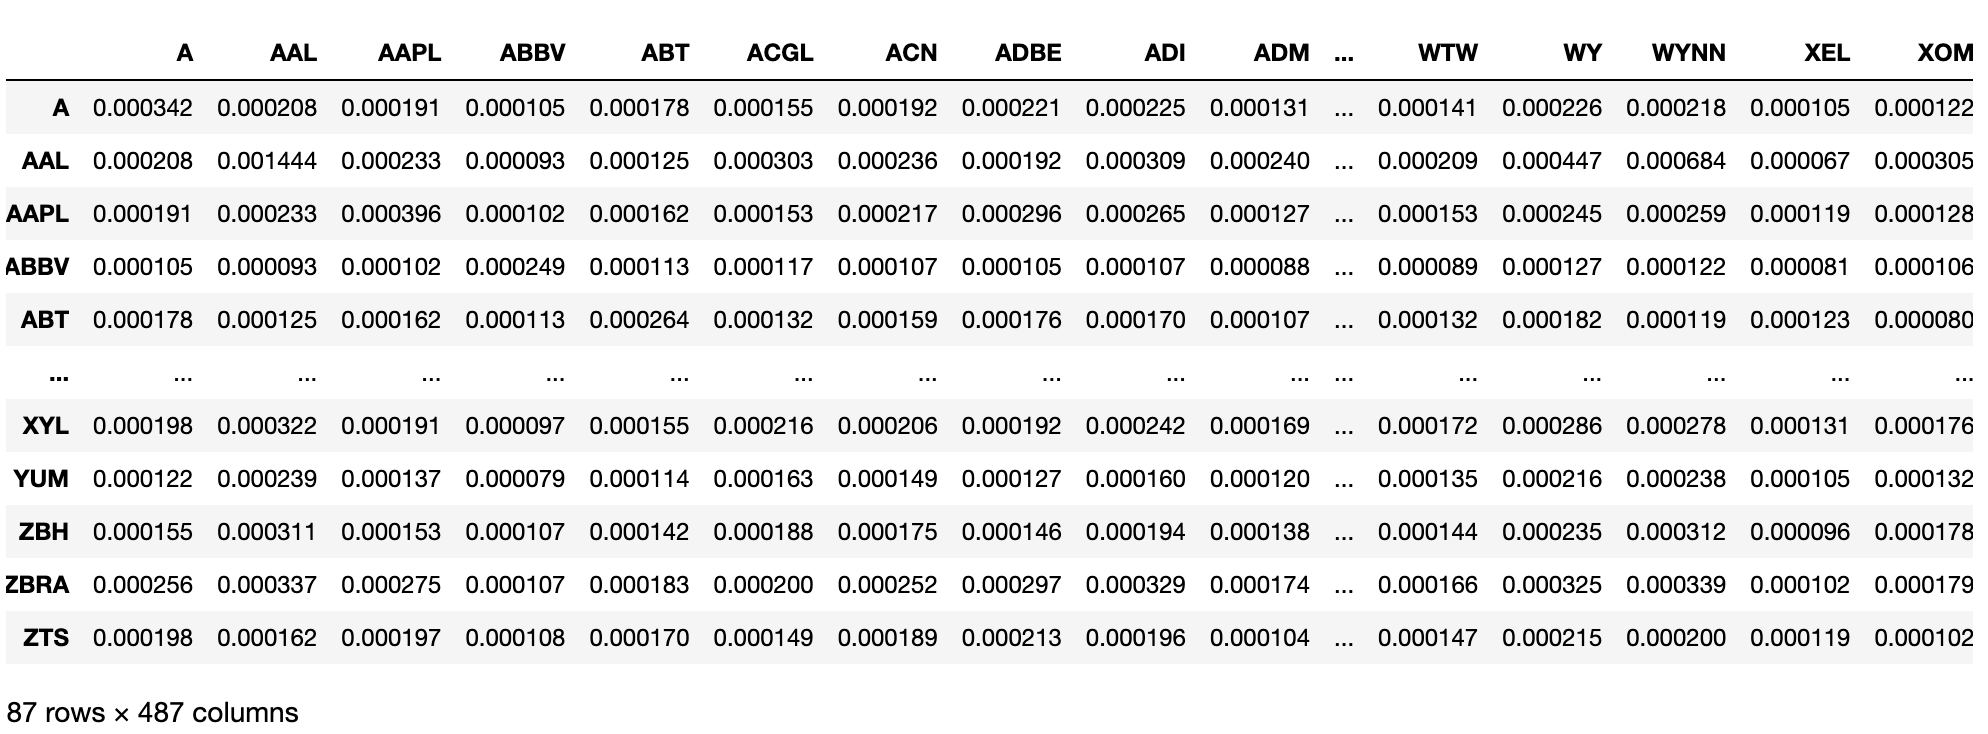
\includegraphics[scale = 0.3]{cov.png}
\end{center}
\end{frame}

\section{Principal Component Analysis}

\begin{frame}
\frametitle{Eigenvectors and -values}
From the spectral theorem, we know that $\Sigma$ is diagonalizable, since it is symmetric. If $\Sigma$ is $k\times k$, and the respective eigenvectors and -values are $v_1, v_2,\ldots, v_k$ and $\lambda_1, \lambda_2,\ldots, \lambda_k$. Then the total variance is $\lambda_1 + \lambda_2+\ldots+\lambda_k$, and the fraction of variance explained by eigenvector $v_i$ is
$$
\frac{\lambda_i}{\lambda_1 +\lambda_2+\ldots+\lambda_i+\ldots+\lambda_k}.
$$
\end{frame}

\begin{frame}[t]
\frametitle{Eigenvectors and -values Example}
\begin{Example}
Consider $\Sigma = \left(\begin{array}{c c} 1	&	0.5\\ 0.5 & 1\end{array}\right)$. Find the eigenvectors and -values.
\end{Example}

\end{frame}

\begin{frame}
\frametitle{Principal Component Analysis}
{\bf Principal component analysis (PCA)} is a dimension reduction technique. It explains some of the variance of the original data in terms of a few eigenvectors with the largest eigenvalues. 

\end{frame}

\begin{frame}
\frametitle{Principal Component Analysis Figure}

\begin{center}
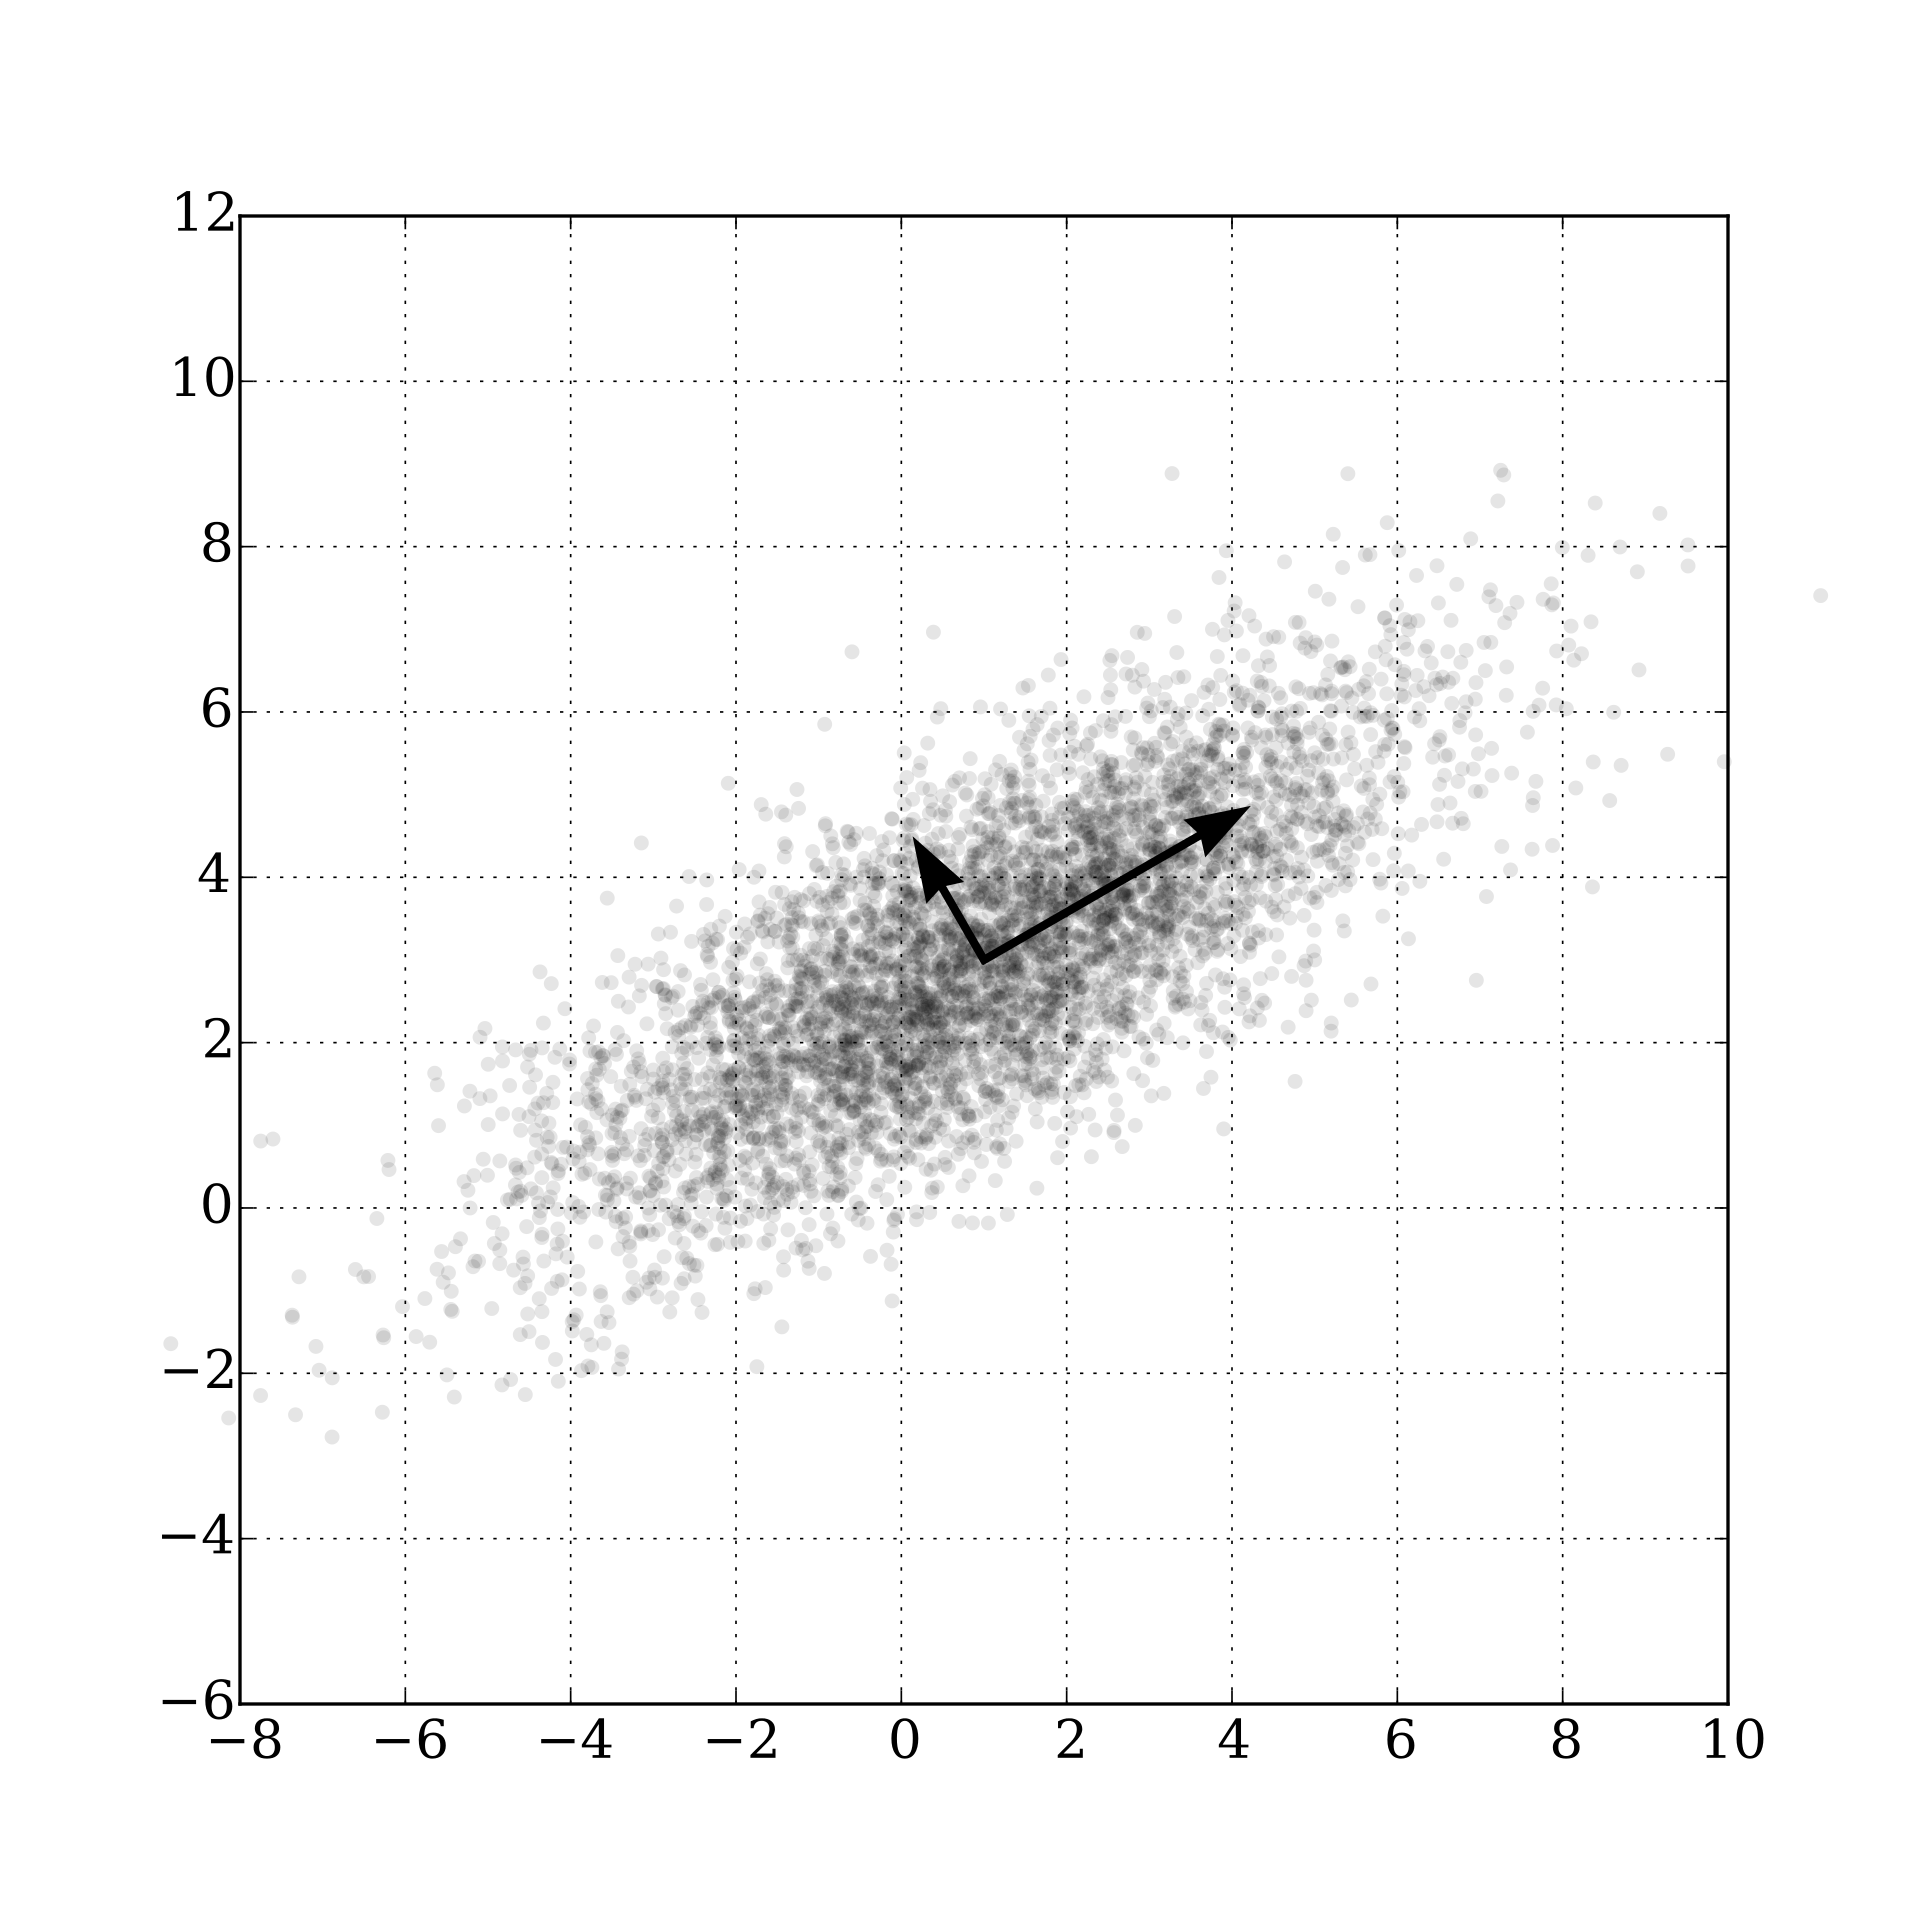
\includegraphics[scale = 0.1]{PCA_fig.png}
\end{center}
\end{frame}

\begin{frame}
\frametitle{Principal Component Analysis Steps}

\begin{enumerate}
\item[1.] Collect your data.
\item[2.] Standardize or demean your data.
\item[3.] Determine how much of the variance you need to explain or how many components are usable for your project.
\item[4.] Get the orthonormal basis of eigenvectors and -values.
\item[5.] Subset the orthonormal basis to the vectors corresponding to the largest $\ell$ eigenvalues, where the value of $\ell$ is based on 3.
\item[6.] Calculate the ``loadings" of each observation on the remaining basis elements.
\end{enumerate}
\end{frame}

\begin{frame}
\frametitle{Convention}
Let's assume that 
$$
i < j\qquad\text{implies}\qquad \lambda_i \geq \lambda_j.
$$ 
In other words, we've rearrange our eigenvalues and corresponding eigenvectors so that the eigenvalues are in descending order.
\end{frame}

\begin{frame}
\frametitle{What are Loadings?}
\small
Suppose $\Sigma$'s eigenvectors are the orthonormal eigenbasis $(v_1, v_2,\ldots, v_k)$. Then observation $u$ can be written as
$$
u = \alpha_1 v_1 + \alpha_2 v_2 +\ldots + \alpha_\ell v_\ell+ \ldots +\alpha_k v_k\qquad\text{where}\qquad \alpha_i = \frac{u \bullet v_i}{\|v_i\|^2} = u \bullet v_i.
$$
We say that $u$ has a {\bf loading} of $\alpha_i$ on $v_i$.

If we subset the basis to the first $\ell$ components, then we would represent $u$ via the vector
$$
\left(\begin{array}{c} \alpha_1\\ \alpha_2\\ \vdots\\ \alpha_\ell \end{array}\right).
$$

\end{frame}

\begin{frame}[fragile]
\frametitle{Principal Component Analysis Example}
\begin{Example}
Use PCA to represent the 100 portfolios from before on a two dimensional scatter plot.
\end{Example}
\begin{multicols}{2}
{
\linespread{0.8}
\tiny
\begin{verbatim*}
import numpy as np
import matplotlib.pyplot as plt

# Use Seaborn style
plt.style.use('seaborn')

# S and data are as calculated previously

# Get the eigenvalues and eigenvectors
evals, evecs = np.linalg.eigh(S)

# Indices in descending order
idx = evals.argsort()[::-1]

# Change order
evecs, evals = evecs[idx], evals[idx]

# Convert the observations to a numpy array
X = data.values

# Get the mean of each industry
x_bar = X.mean(axis = 0)

# Demean X
X -= x_bar

# Calculate loadings using the dot product
loadings = X @ evecs[:, 0:2]

# Unpack results
x, y = zip(*loadings)

# Get scatter plot
plt.scatter(x, y)

# Create x- and y-labels
plt.xlabel('PCA1')
plt.ylabel('PCA2')

# Give the plot a title
plt.title('100 Portfolios Data with Dimension 
     Reduction')

# Save the figure
plt.savefig(r'[location of file]')

plt.show()
\end{verbatim*}
}
\end{multicols}
\end{frame}

\begin{frame}
\frametitle{Principal Component Analysis Result}
\begin{center}
\includegraphics[scale = 0.4]{ex16.png}
\end{center}

\end{frame}

\begin{frame}
\frametitle{Reconstruction}
If we have data with mean $\mu$, and we used the loadings of the first $\ell$ eigenvectors $v_1, v_2,\ldots, v_\ell$ to approximate $u$, then this is making the assumption
$$
u \approx \mu + \alpha_1 v_1 + \alpha_2 v_2+\ldots + \alpha v_\ell,
$$
where $\alpha_i$ is the loading corresponding to $v_i$. 

\end{frame}

\begin{frame}
\frametitle{Why Standardize?}
PCA results are affected by the scale of your data. However, in many applications scale is already known and users are more interested in correlations within the data. 
\end{frame}

\section{Clipping Covariance Matrix}

\begin{frame}
\frametitle{Positive Definite Matrix}
Using the dot product, a matrix $S$ is {\it positive definite} if
$$
x^T S x > 0 \qquad\text{for all}\qquad x \neq O.
$$
Since a covariance matrix is diagonalizable due to the spectral theorem, a covariance matrix will be positive definite if and only if all its eigenvalues are positive.
\end{frame}

\begin{frame}
\frametitle{Negative and Zero Eigenvalues}

\begin{itemize}
\item When $S$ is a covariance matrix, it never makes sense to have negative eigenvalues. These results are simply numerical errors.
\item A zero eigenvalue indicates one variable can be written as a linear combination of the others, which may or may not make sense given the context.
\end{itemize}

\end{frame}

\begin{frame}[fragile]
\frametitle{Negative and Zero Eigenvalues Example}
%\begin{multicols}{2}
{
\linespread{0.8}
\tiny
\begin{verbatim*}
# Import modules
import numpy as np
import matplotlib.pyplot as plt
from scipy.stats import norm

# Set the random seed
np.random.seed(0)

# Generate normal random variables
X = norm.rvs(size = (50, 100))

# Get the covariance matrix
S = np.cov(X, rowvar = False)

# Get the eigenvalues
evals, _ =  np.linalg.eigh(S)

print(f'The sample covariance matrix has {np.sum(evals <= 0)} eigenvalues less than or equal to 0.')
\end{verbatim*}
}
%\end{multicols}

It says there are 24 eigenvalues less than or equal to 0! The true covariance matrix  is $I$ and therefore only has positive eigenvalues. 
\end{frame}

\begin{frame}
\frametitle{Clip Covariance Matrix}

One solution is to ``clip" the sample covariance matrix. Simply replace all the eigenvalues that are too small with something bigger and reconstruct the covariance matrix.

\end{frame}

\begin{frame}[fragile]
\frametitle{Clip Covariance Matrix Example}
\small
Using the results from before. 
\begin{multicols}{2}
{
\linespread{0.8}
\tiny
\begin{verbatim*}
# Get the standard deviations
stds = np.sqrt(np.diag(S))

# Get the correlation matrix
C = np.diag(1/stds) @ S @ np.diag(1/stds)

# Get the eigenvalues and vectors of C
evals_c, evecs_c = np.linalg.eigh(C)

# Round to 14 decimal places 
# Avoids numerical problems
evals_new = np.round(evals_c, 14)

# Define minimum eigenvalue
lam_min = np.min(evals_new[evals_new > 0])

# Replace with smallest positive
evals_new[evals_new < lam_min] = lam_min

# Reconstruct correlation matrix
C_new = evecs_c @ np.diag(evals_new) @ evecs_c.T

# Make sure still correlation matrix
C_new = (np.diag(np.sqrt(1/np.diag(C_new))) @ C_new
            @ np.diag(np.sqrt(1/np.diag(C_new))))

# Multiply by standard deviations 
# Makes it covariance matrix
S_new = np.diag(stds) @ C_new @ np.diag(stds)

# Get the eigenvalues
evals_new, _ =  np.linalg.eigh(S_new)

print(f'The new covariance matrix estimate has 
{np.sum(evals_new <= 0)} eigenvalues less than 
or equal to 0.')
\end{verbatim*}
}
\end{multicols}

Now it says all the eigenvalues are positive! Inspection shows that the covariance matrix estimate is otherwise very similar to the sample covariance matrix.
\end{frame}

\begin{frame}
\frametitle{Marchenko-Pastur Theorem}
\small
\begin{Theorem}
Consider a matrix of independent and identically distributed random observations $X$ of size $T\times N$, where the underlying process generating the observations has mean 0 and variance $\sigma^2$. If $q = T/N > 1$ is constant, the matrix $C = \frac{1}{T} X^T X$ has eigenvalues that converges to a distribution with probability density function
$$
f(\lambda) = \begin{cases} \frac{q}{2\pi\sigma^2} \frac{\sqrt{(\lambda_+ - \lambda)(\lambda - \lambda_-)}}{\lambda}, & \lambda_- \leq \lambda \leq \lambda_+\\ 0, & \text{otherwise}\end{cases}
$$
where
$$
\lambda_- = \sigma^2 \left(1 - \sqrt{\frac{1}{q}}\right)^2\qquad\text{and}\qquad \lambda_+ = \sigma^2 \left(1 + \sqrt{\frac{1}{q}}\right)^2.
$$
\end{Theorem}
\end{frame}

\begin{frame}[fragile]
\frametitle{Marchenko-Pastur Example}

\begin{multicols}{2}

\linespread{0.8}
\tiny
\begin{verbatim*}
# Import modules
import numpy as np
import matplotlib.pyplot as plt
from scipy.stats import norm

# Use latex
plt.rcParams['text.usetex'] = True

# Use Seaborn style
plt.style.use('seaborn')

# Set the random seed
np.random.seed(0)

# Generate normal random variables
X = norm.rvs(size = (10000, 1000))

# Get the number of observations and variables
T, N = X.shape

# Get correlation matrix
C = np.corrcoef(X, rowvar = False)

# q is obs/vars
q = T/N

# Get eigenvalues
evals, _ = np.linalg.eigh(Corr)

# Get support of Marchenko–Pastur distribution
lam_minus = (1 - np.sqrt(1/q))**2,
lam_plus = (1 + np.sqrt(1/q))**2 

# Define pdf
def f(lam):
    
    # If in support... 
    if lam_minus <= lam <= lam_plus:
        
        factor1 = q/(2 * np.pi)
        factor2 = np.sqrt((lam_plus - lam) 
          * (lam - lam_minus))/lam
        
        return factor1 * factor2
     
     # Outside of support...          
    else:
                
        return 0

# Get lam_vals
lam_vals = np.linspace(lam_minus, lam_plus, 100)

# Get density values
f_vals = [f(lam) for lam in lam_vals]
\end{verbatim*}

\end{multicols}

\end{frame}

\begin{frame}[fragile]
\frametitle{Marchenko-Pastur Example Cont.}

{
\linespread{0.8}
\tiny
\begin{verbatim*}
# Plot histogram
plt.hist(evals, density = True, bins = int(np.sqrt(N)), label = 'Simulated Distribution')

# Plot density
plt.plot(lam_vals, f_vals, label = 'Density')

# Add legend
plt.legend()

# Add x-label
plt.xlabel(r'$\lambda$')

# Add y-label
plt.ylabel(r'Density')

# Add title to plot
plt.title(r'Marchenko–Pastur Distribution')

# Save the figure
plt.savefig(r'[location on machine]')

plt.show()
\end{verbatim*}
}

\end{frame}

\begin{frame}[fragile]
\frametitle{Marchenko-Pastur Result}

\begin{center}
\includegraphics[scale = 0.5]{ex17.png}
\end{center}

\end{frame}

\begin{frame}
\frametitle{How to use it?}
Consider eigenvalue $\lambda$ of the covariance matrix.
\begin{itemize}
\item If $\lambda > \lambda_+$, then result consistent with signal. 
\item If $\lambda \leq \lambda_+$, the result is probably just random noise. Replace values less than $\lambda_+$ with mean of values less than $\lambda_+$.
\end{itemize}

\end{frame}

\begin{frame}[fragile]
\frametitle{100 Portfolio Example}
Suppose we have the ``100 Portfolios Formed on Size and Book-to-Market" data from before.
\begin{multicols}{2}{
\linespread{0.8}
\tiny
\begin{verbatim*}
# Save q
q = data.shape[0]/data.shape[1]

# Get covariance matrix; convert to numpy array
S = data.cov().values

# Get the standard devations
stds = np.sqrt(np.diag(S))

# Calculate correlation matrix
C = np.diag(1/stds) @ S @ np.diag(1/stds)

# Get support of Marchenko–Pastur distribution
lam_minus = (1 - np.sqrt(1/q))**2
lam_plus = (1 + np.sqrt(1/q))**2

# Get the eigenvalues and eigenvectors
evals, evals =  np.linalg.eigh(C)

# Define pdf
def f(lam):
    # If in support... 
    if lam_minus <= lam <= lam_plus:       
        factor1 = q/(2 * np.pi)
        factor2 = np.sqrt((lam_plus - lam) 
          * (lam - lam_minus))/lam     
        return factor1 * factor2
     # Outside of support...          
    else:            
        return 0

# Get lam_vals
lam_vals = np.linspace(lam_minus, lam_plus, 100)

# Get density values
f_vals = [f(lam) for lam in lam_vals]

# Plot histogram
plt.scatter(evals, np.zeros(len(evals)), 
     label = 'Eigenvalues')
# Plot density
plt.plot(lam_vals, f_vals, label = 'Density', 
     color = 'green')
# There is an eigenvalue at 70 which messes up graph
plt.xlim([0, 4])
# Add legend
plt.legend()
# Add x-label
plt.xlabel(r'$\lambda$')
# Add y-label
plt.ylabel(r'Density')
# Add title to plot
plt.title(r'100 Portfolios')
# Save the figure
plt.savefig(r'[location on machine]')
plt.show()
\end{verbatim*}
\end{multicols}
\end{frame}

\begin{frame}[fragile]
\frametitle{100 Portfolio Example}
Only the values past $\lambda_+$ are consistent with signal. There is an eigenvalue of about 70 that is not shown.
\begin{center}
\includegraphics[scale = 0.4]{ex18.png}
\end{center}

\end{frame}


\begin{frame}[fragile]
\frametitle{Clip Matrix}
{
\linespread{0.8}
\tiny
\begin{verbatim*}
# Initialize new eigenvalues
evals_new = evals

# Replace noise eigenvalues with mean
evals_new[evals_new < lam_plus] = np.mean(evals_new[evals_new < lam_plus])

# Construct new correlation matrix
C_new = evecs @ np.diag(evals_new) @ evecs.T

# Make sure still correlation matrix
C_new = np.diag(1/np.sqrt(np.diag(C_new))) @ C_new @ np.diag(1/np.sqrt(np.diag(C_new)))

# Make new covariance matrix
S_new = np.diag(stds) @ C_new @ np.diag(stds)
\end{verbatim*}
}
\end{frame}





\end{document}
